\documentclass[border=4pt]{standalone}
% Shared typography and colours for the standalone figures.
\usepackage{unicode-math}
\setmainfont{TeX Gyre Termes}
\setmathfont{TeX Gyre Termes Math}
\usepackage{tikz}
\usetikzlibrary{arrows.meta,positioning,calc,decorations.pathreplacing}
\usepackage{pgfplots}
\pgfplotsset{compat=1.18}

% One colour per element or subsystem. Record the mapping in
% the working repository conventions and use it identically in every figure.
\definecolor{elemA}{HTML}{1F5FA8}
\definecolor{elemB}{HTML}{B8461B}
\definecolor{elemC}{HTML}{2E7D32}
\definecolor{elemD}{HTML}{6A4C93}
\definecolor{frameline}{HTML}{555555}

% Article-specific diagram styling; common figure-style.tex remains managed.
\usepackage{circuitikz}
\usetikzlibrary{decorations.pathmorphing,fit,backgrounds}
\tikzset{
  every node/.style={font=\small},
  block/.style={draw=frameline,rounded corners=2pt,minimum height=7mm,align=center,fill=white},
  massA/.style={draw=elemA,fill=elemA!10,thick},
  massB/.style={draw=elemB,fill=elemB!10,thick},
  receiver/.style={draw=elemC,fill=elemC!9,thick},
  mediator/.style={draw=elemD,fill=elemD!8,thick},
  flow/.style={-{Latex[length=2.3mm]},thick},
  boundary/.style={draw=frameline,dashed,rounded corners=3pt},
  spring/.style={decorate,decoration={coil,aspect=.4,segment length=3mm,amplitude=1.5mm},thick,elemD}
}

\begin{document}
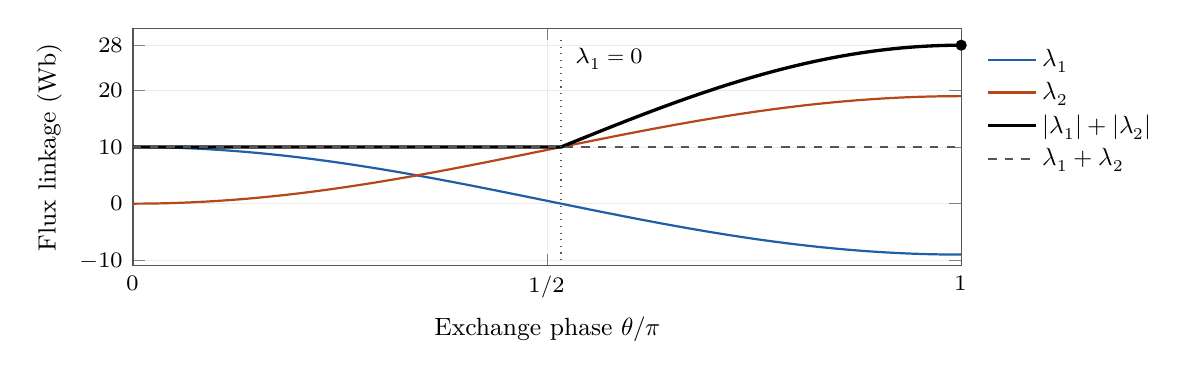
\begin{tikzpicture}
\begin{axis}[
 width=12.1cm,height=4.6cm,
 xmin=0,xmax=1,ymin=-11,ymax=31,
 xlabel={Exchange phase $\theta/\pi$},ylabel={Flux linkage (Wb)},
 xtick={0,.5,1},xticklabels={$0$,$1/2$,$1$},
 ytick={-10,0,10,20,28},
 grid=major,grid style={frameline!12},
 axis line style={frameline},
 tick label style={font=\footnotesize},
 label style={font=\small},
 legend style={at={(1.02,.96)},anchor=north west,draw=none,font=\footnotesize},
 legend cell align=left,
 samples=121,domain=0:1,
]
\addplot[thick,elemA] {(1+19*cos(180*x))/2};
\addlegendentry{$\lambda_1$}
\addplot[thick,elemB] {19*(1-cos(180*x))/2};
\addlegendentry{$\lambda_2$}
\addplot[very thick,black] {abs((1+19*cos(180*x))/2)+19*(1-cos(180*x))/2};
\addlegendentry{$|\lambda_1|+|\lambda_2|$}
\addplot[dashed,thick,frameline] {10};
\addlegendentry{$\lambda_1+\lambda_2$}
\draw[dotted,frameline] (axis cs:{acos(-1/19)/180},-10)--(axis cs:{acos(-1/19)/180},29);
\node[font=\footnotesize,anchor=north west,fill=white,inner sep=1pt]
 at (axis cs:.53,28) {$\lambda_1=0$};
\addplot[only marks,mark=*,mark size=1.8pt,black] coordinates {(1,28)};
\end{axis}
\end{tikzpicture}
\end{document}
